\documentclass[english]{maciarticle}

\usepackage{amsmath,amsbsy,amscd,amssymb,graphicx, epsfig,color,float}
\usepackage[numbers,sort&compress]{natbib} 

%%%%%%%%%%%%%%%%%%%%%%%%%%%%%%%%%%%%%%%%%%%%%
\begin{document}

\title{Hierarchical Risk Parity for Cryptocurrency Portfolios: A Comparative Analysis}

\author[$\flat$]{Alan Matys}
\author[$\dag$]{Federico Martin Rodriguez}
\affil[$\flat$]{Universidad del CEMA,
\textcolor{blue} {alan.matys92@gmail.com, federico.m.rodriguez.h@gmail.com}}
s
\maketitle

\begin{abstract}
This article addresses portfolio construction as a budget allocation problem, balancing expected returns with risk mitigation. Traditional methods like the Critical Line Algorithm (CLA) struggle with diversification due to their sensitivity to input parameters. Hierarchical Risk Parity (HRP) offers a robust alternative by employing correlation-based clustering and hierarchical weight allocation. We evaluate HRP’s effectiveness in cryptocurrency markets, where traditional optimization methods face challenges due to high volatility and inter-asset correlations. Our findings demonstrate that HRP achieves superior diversification while maintaining computational stability, making it a compelling choice for risk-based asset allocation.
\end{abstract}

\begin{keywords}
Hierarchical Risk Parity, Risk-based asset allocation, Cryptocurrency, Portfolio Optimization
\end{keywords}

\begin{mathsubclass}
21A54 - 55P54
\end{mathsubclass}

{\thispagestyle{empty}} %DO NOT DELETE THIS LINE

%%===============================
\section{Introduction}
%%===============================

Portfolio construction is a fundamental problem in finance and investment management, where capital is allocated across different assets to balance expected return and risk. Traditional mean-variance optimization, pioneered by \citet{markowitz1952portfolio}, provides a theoretically optimal solution by minimizing variance given expected returns. However, this approach heavily relies on accurate estimations of return and covariance matrices, which can introduce significant instability in real-world applications.

The \textbf{Critical Line Algorithm (CLA)} by Markowitz is one of the most widely used methods for portfolio optimization. While it ensures weight convergence after a finite number of steps, it is sensitive to estimation errors, often resulting in concentrated allocations and poor out-of-sample performance \citep{lopez2016}. Furthermore, inverting the covariance matrix can lead to numerical instability, particularly when dealing with highly correlated assets.

To address these issues, alternative portfolio allocation strategies have emerged. Among them, \textbf{Hierarchical Risk Parity (HRP)} offers a robust, data-driven approach that leverages clustering techniques to construct diversified portfolios. Unlike traditional methods, HRP does not require matrix inversion, making it computationally stable even in cases of singular covariance matrices \citep{lopez2018}. In this work, we evaluate HRP’s performance in cryptocurrency markets, a domain characterized by extreme volatility and strong inter-asset correlations.

%%===============================
\section{HRP Portfolio Building}
%%===============================

HRP follows a three-step process to allocate portfolio weights. First, hierarchical clustering groups assets based on their correlation structure. This is followed by quasi-diagonalization, where assets are reordered to reflect their relative risk profiles. Finally, recursive bisection distributes weights across the asset hierarchy, ensuring a balanced allocation.

The hierarchical clustering step constructs a distance matrix from asset correlations:

\[
d_{i,j} = \sqrt{\frac{1}{2}(1 - \rho_{i,j})}.
\]

where \(\rho_{i,j}\) is the Pearson correlation coefficient between assets \(X_i\) and \(X_j\). The distance matrix is then used to compute a linkage tree, which serves as the basis for asset clustering.

In the quasi-diagonalization step, assets are reordered such that strongly correlated assets appear closer together. This ensures that risk is more evenly distributed in the final portfolio. The recursive bisection step applies an inverse-variance weighting scheme within each cluster, progressively allocating weights in a top-down manner.

%%===============================
\section{Results and Evaluation Methodology}
%%===============================

The proposed methodology is tested against traditional allocation techniques, including the \textbf{Inverse Variance Portfolio (IVP)} and the \textbf{Minimum Variance Portfolio (MVP)}, as well as a simple strategy of holding Bitcoin (BTC) and Ethereum (ETH) throughout the backtesting period. The backtest spans from \textbf{January 1, 2021, to December 31, 2023}.

Two allocation scenarios are considered. First, a \textbf{Static Portfolio Allocation}, where weights are assigned once at the start of the backtest and remain unchanged. Second, a \textbf{Monthly Rebalancing} scenario, where portfolios are reweighted at the start of each month, incorporating a transaction cost rate of **0.1\% per trade**.

Performance is evaluated using key portfolio metrics:

\textbf{Total Return (\%)} measures the cumulative percentage gain or loss over the period.  
\textbf{Annualized Volatility (\%)} quantifies the standard deviation of returns on an annualized basis.  
\textbf{Sharpe Ratio} assesses risk-adjusted returns, comparing excess returns relative to volatility. Here, the risk-free rate is assumed to be **0**.  
\textbf{Sortino Ratio} is similar to the Sharpe Ratio but considers only downside risk.  
\textbf{Maximum Drawdown (\%)} represents the largest peak-to-trough decline in portfolio value.  
\textbf{Calmar Ratio} compares total return to maximum drawdown, providing a measure of risk-adjusted performance.

\subsection{Final Results}

Figure \ref{fig:static_cum_returns} presents the cumulative returns for the **Static Portfolio Allocation** scenario, while Table \ref{tab:static_metrics} summarizes the performance metrics.

\begin{figure}[H]
    \centering
    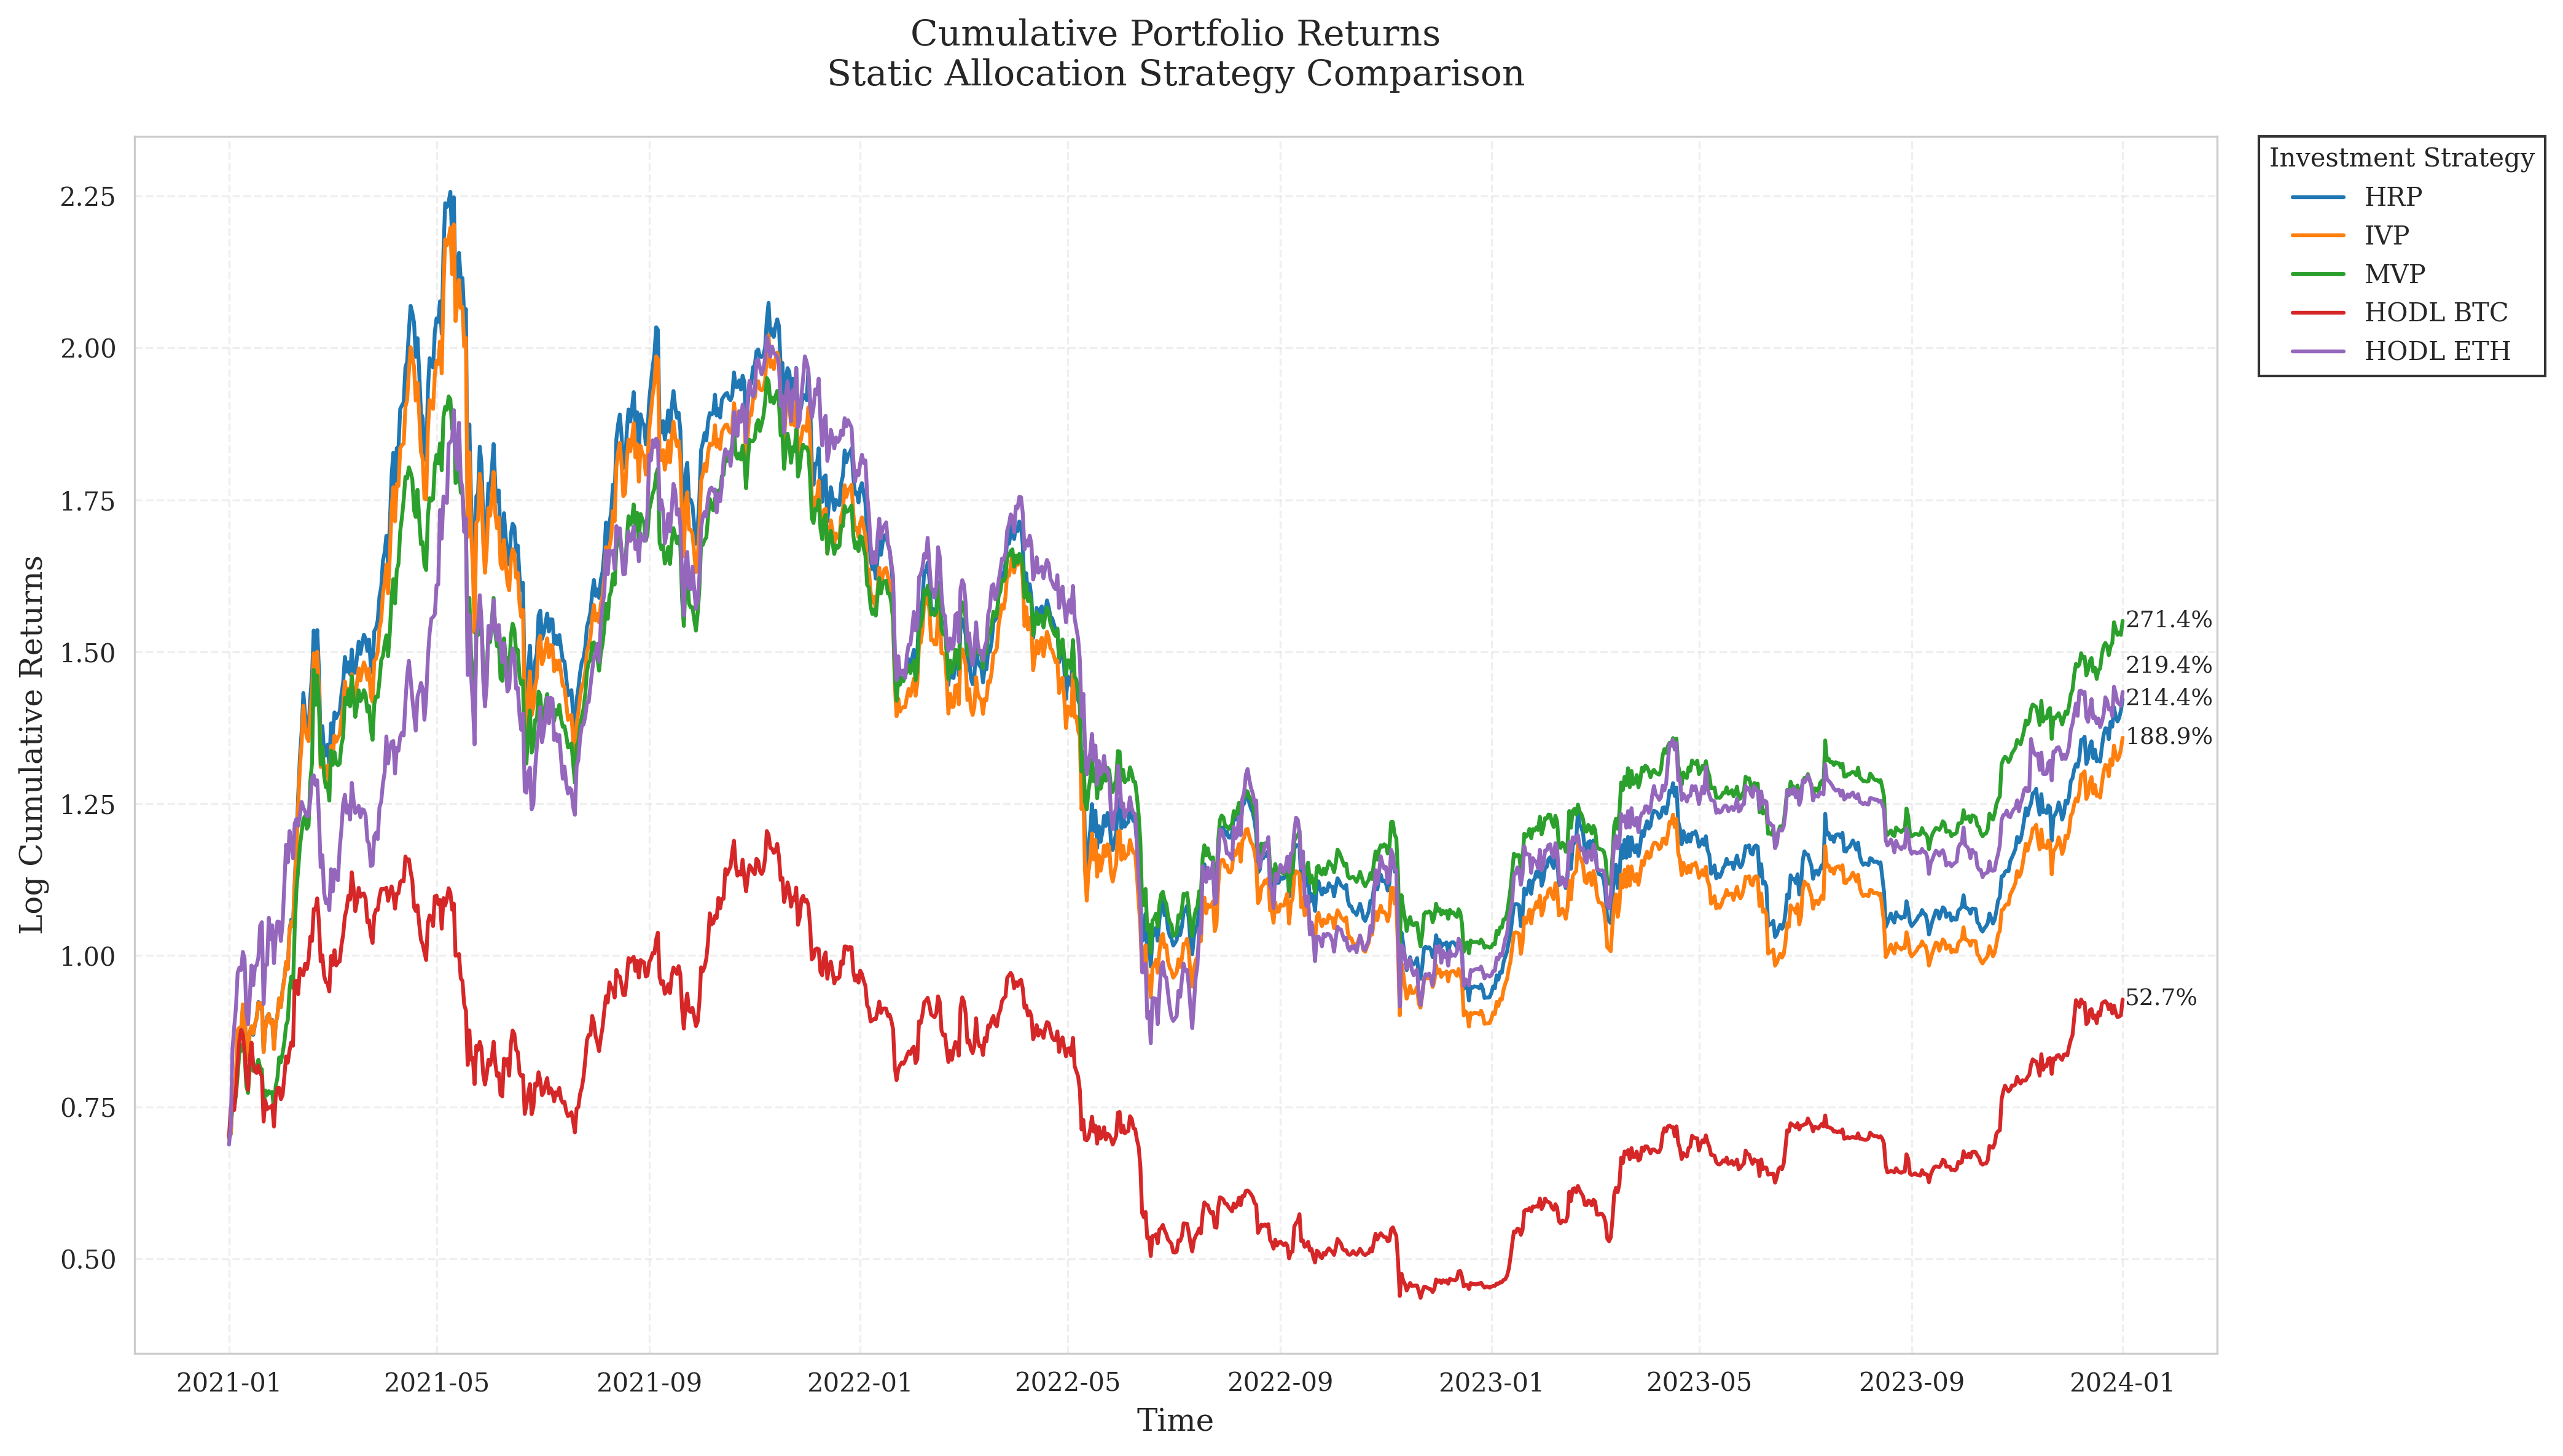
\includegraphics[width=0.8\textwidth]{static_cumulative_returns.png}
    \caption{Cumulative Returns for Static Portfolio Allocation.}
    \label{fig:static_cum_returns}
\end{figure}

\begin{table}[H]
    \centering
    \caption{Performance Metrics for Static Portfolio Allocation}
    \label{tab:static_metrics}
    \small
    \begin{tabular}{|l|c|c|c|c|c|c|}
    \hline
    Portfolio & Total Return (\%) & Volatility (\%) & Sharpe Ratio & Sortino Ratio & Max Drawdown (\%) & Calmar Ratio \\
    \hline
    HRP & 214.45 & 82.17 & 0.88 & 0.82 & -82.21 & 0.57 \\
    IVP & 188.86 & 82.07 & 0.85 & 0.79 & -82.42 & 0.51 \\
    MVP & 271.45 & 70.51 & 0.97 & 0.98 & -71.38 & 0.77 \\
    BTC & 52.75 & 64.86 & 0.54 & 0.57 & -76.63 & 0.20 \\
    ETH & 219.39 & 84.68 & 0.88 & 0.91 & -79.30 & 0.60 \\
    \hline
    \end{tabular}
\end{table}

Similar results for the **Monthly Rebalancing** scenario are shown in Figure \ref{fig:rebalance_cum_returns} and Table \ref{tab:rebalance_metrics}.

%%===============================
\section{Conclusion}
%%===============================

This study demonstrates that HRP provides a computationally stable and well-diversified alternative to traditional portfolio optimization techniques. Compared to CLA-based methods, HRP achieves superior risk-adjusted performance, particularly in high-volatility environments such as cryptocurrency markets. Future research should explore denoising techniques to mitigate small eigenvalue distortions in correlation matrices and investigate methods to reduce the impact of market-wide correlation shocks.

%%===============================
\section*{References}
%%===============================

\begin{thebibliography}{9}

\bibitem{markowitz1952portfolio}
Markowitz, H. (1952). \textit{Portfolio Selection}. The Journal of Finance, 7(1), 77–91. \texttt{https://doi.org/10.2307/2975974}

\bibitem{lopez2016}
López de Prado, M. (2016). \textit{Building Diversified Portfolios that Outperform Out-of-Sample}. Journal of Portfolio Management. \texttt{https://doi.org/10.3905/jpm.2016.42.4.059}

\bibitem{lopez2018}
López de Prado, M. (2018). \textit{Advances in Financial Machine Learning}. John Wiley \& Sons.

\bibitem{lopez2020}
López de Prado, M. (2020). \textit{Machine Learning for Asset Managers}. Cambridge University Press.

\end{thebibliography}

\end{document}